\section{The logistic regression model}\label{sec:logist-model}

The logistic regression model
describes the relationship between a categorical outcome variable,
the ``response'', and a set of explanatory variables.
The response variable is often \boldital{dichotomous}, although
extensions to the model permit multi-category,
\boldital{polytomous} outcomes, discussed in
\secref{sec:logist-poly}.
The explanatory variables may be continuous or (with dummy variables)
discrete.

For a binary response, $Y$, and a continuous explanatory variable, $X$,
we may be interested in modeling the probability of a successful
outcome, which we denote $\pi(x) \equiv \Pr(Y=1 \given X=x)$.
That is, at a given value $X = x$, we imagine that there is a
binomial distribution of the responses, $\Bin( \pi(x), n_x )$.

We might contemplate a simple linear regression model for $\pi(x)$,
\begin{equation*}%\label{eq:logit0}
E ( Y ) = \pi(x) =
\alpha + \beta x \comma
\end{equation*}
which we could fit by ordinary least squares (\PROC{REG}, for example).
However, such a model (called the \emph{linear probability model}),
has the serious defect that it yields predicted probabilities $\hat{\pi}(x) < 0$
for sufficiently small $x$ and $\hat{\pi}(x) > 1$ for sufficiently large $x$
(assuming $\beta > 0$).

One way around this difficulty is to re-specify the model so that a
transformation of $\pi$ has a linear relation to $x$, and that transformation
keeps $\hat{\pi}$ between 0 and 1 for all $x$.
A particularly convenient choice gives the linear logistic regression model, which posits a linear relation between
the log odds, or \glossterm{logit} of this probability and $X$,
\begin{equation}\label{eq:logit1}
\logit[ \pi(x) ] \equiv
\log \left( \frac{\pi(x) }{1-\pi(x) } \right) =
\alpha + \beta x \period
\end{equation}
When $\beta > 0$, $\pi (x)$ and the log odds increase as $X$ increases;
when $\beta < 0$ they decrease with $X$.
From \eqref{eq:logit1} we see that the odds of a favorable response
can be expressed as
%
\begin{equation}\label{eq:logit2}
\mbox{odds}(Y=1) \equiv \frac{\pi(x) }{1-\pi(x) }  =
\exp (\alpha + \beta x) = e^{\alpha} ( e^{\beta} )^x \: ,
\end{equation}
%
a multiplicative model for the odds.
So, under the logistic model,
\begin{itemize*}
\item $\beta$ is the change in the log odds associated with a unit
increase in $x$.
The odds are multiplied by $e^{\beta}$ for each unit increase in $x$.
\item $\alpha$ is log odds at $x=0$; $e^{\alpha}$ is the odds of
a favorable response at this $x$-value
(which may not have a reasonable interpretation if $X=0$ is far from
the range of the data).
\end{itemize*}

Rearranging terms in \eqref{eq:logit2}, the logistic regression model may also be formulated as a direct relationship for the probability of success,
\begin{equation}\label{eq:logit3}
\pi(x) = \frac{\exp (\alpha + \beta x)}{1+ \exp (\alpha + \beta x) } \:.
\end{equation}
This expression may look complex, but, the numerical results are
easy to interpret.
We will find it most convenient for plotting and understanding results
from logistic regression to express fitted values on the scale of
probabilities.

It may also help to know that, on the scale of probabilities, the 
slope of the relationship between $\pi(x)$ and $x$ is
$\beta \pi (1-\pi)$, so you can also interpret the slope in
\eqref{eq:logit1} as a change in probability of success for a unit
change in $x$. But the numerical value depends on the probability itself.
This expression is at its maximum when $\pi = 0.5$.  However
it doesn't change very much within the range $0.2 < \pi < 0.8$, as we
will see in the following example.

\begin{Example}[arthrit6]{Arthritis treatment}
\begin{table}[htb]
 \caption{Probabilities, Odds, and Logits for the Arthritis Treatment Data}\label{tab:arthlogit}
 \begin{center}
 \begin{tabular}{r@{ -- }l rrrrr}
 \hline
  \multicolumn{2}{c}{Age}
		       & Number &       & Observed   & Odds   & Observed \\ 
  \multicolumn{2}{c}{Group} 
             & Better & Total & $\Pr\{\mbox{Better}\}$ & Better & Logit \\ \hline
  23  &  31  &    2  &   8  &  0.250  &  0.333  &  -1.099 \\ 
  32  &  41  &    4  &   9  &  0.444  &  0.800  &  -0.223 \\ 
  44  &  48  &    2  &   8  &  0.250  &  0.333  &  -1.099 \\ 
  49  &  53  &    0  &   7  &  0.000  &  0.000  &  . \\ 
  54  &  57  &    9  &  12  &  0.750  &  3.000  &   1.099 \\ 
  58  &  58  &    2  &   3  &  0.667  &  2.000  &   0.693 \\ 
  59  &  61  &    7  &  11  &  0.636  &  1.750  &   0.560 \\ 
  62  &  63  &    4  &   8  &  0.500  &  1.000  &   0.000 \\ 
  64  &  67  &    5  &   9  &  0.556  &  1.250  &   0.223 \\ 
  68  &  74  &    7  &   9  &  0.778  &  3.500  &   1.253 \\ 
 \hline
 \end{tabular}
 \end{center}
\end{table}

In \chref{ch:twoway} we examined the data
on treatment for rheumatoid arthritis.
In addition to sex and treatment, the data (see \datref{dat:arthrit})
gives the age of each patient in this study.
Although the response has three categories (none, some, or marked
improvement), for now we consider whether the patient showed any
improvement at all, defining the event ``better'' to be some or
marked improvement.

Because age is continuous, it is difficult to see how the probability of
a better response varies with age.
\tabref{tab:arthlogit} summarizes these data
by dividing the patients into 10 decile groups based on age.%
\footnote{The ``total'' numbers are unequal because of ties.}
We see that for those in the youngest age group the observed
$\Pr\{\textrm{Better}\} = 2/8 = 0.25$, so the odds of a better response
is $0.25 / 0.75 = \frac{1}{3}$;  for those in the 62--63 age range,
half improved, so the odds = 1.  The log odds has the value 0 here.
Thus positive (negative) logits correspond to probabilities greater than
(less than) $\frac{1}{2}$.

You can see that the probabilities of a better response
and the logits tend to increase
with age.  Thus, we would expect to find $\beta > 0$ in Eqn.~\eqref{eq:logit1}.
Also note that when the probability is defined as
the observed number divided by the total in a group, the logit is
undefined when the observed probability is 0 or 1.
We improve on this below.

\figref{fig:logist1c1} shows a plot of the (0/1) variable \texttt{better}
against age.  (The programming for such plots is described in
\secref{sec:logist-quantp}.)
Also shown is the predicted probability from a logistic
regression (solid blue curve) and the upper and lower 95\% confidence
band for this predicted probability (dashed blue curves).
For comparison, we also show the result of a linear regression of
the (0/1) variable on age (red line) and its 95\% confidence band.
The two sets of curves are fairly similar, except in the extremes.
\begin{figure}[htb]
  \centering
  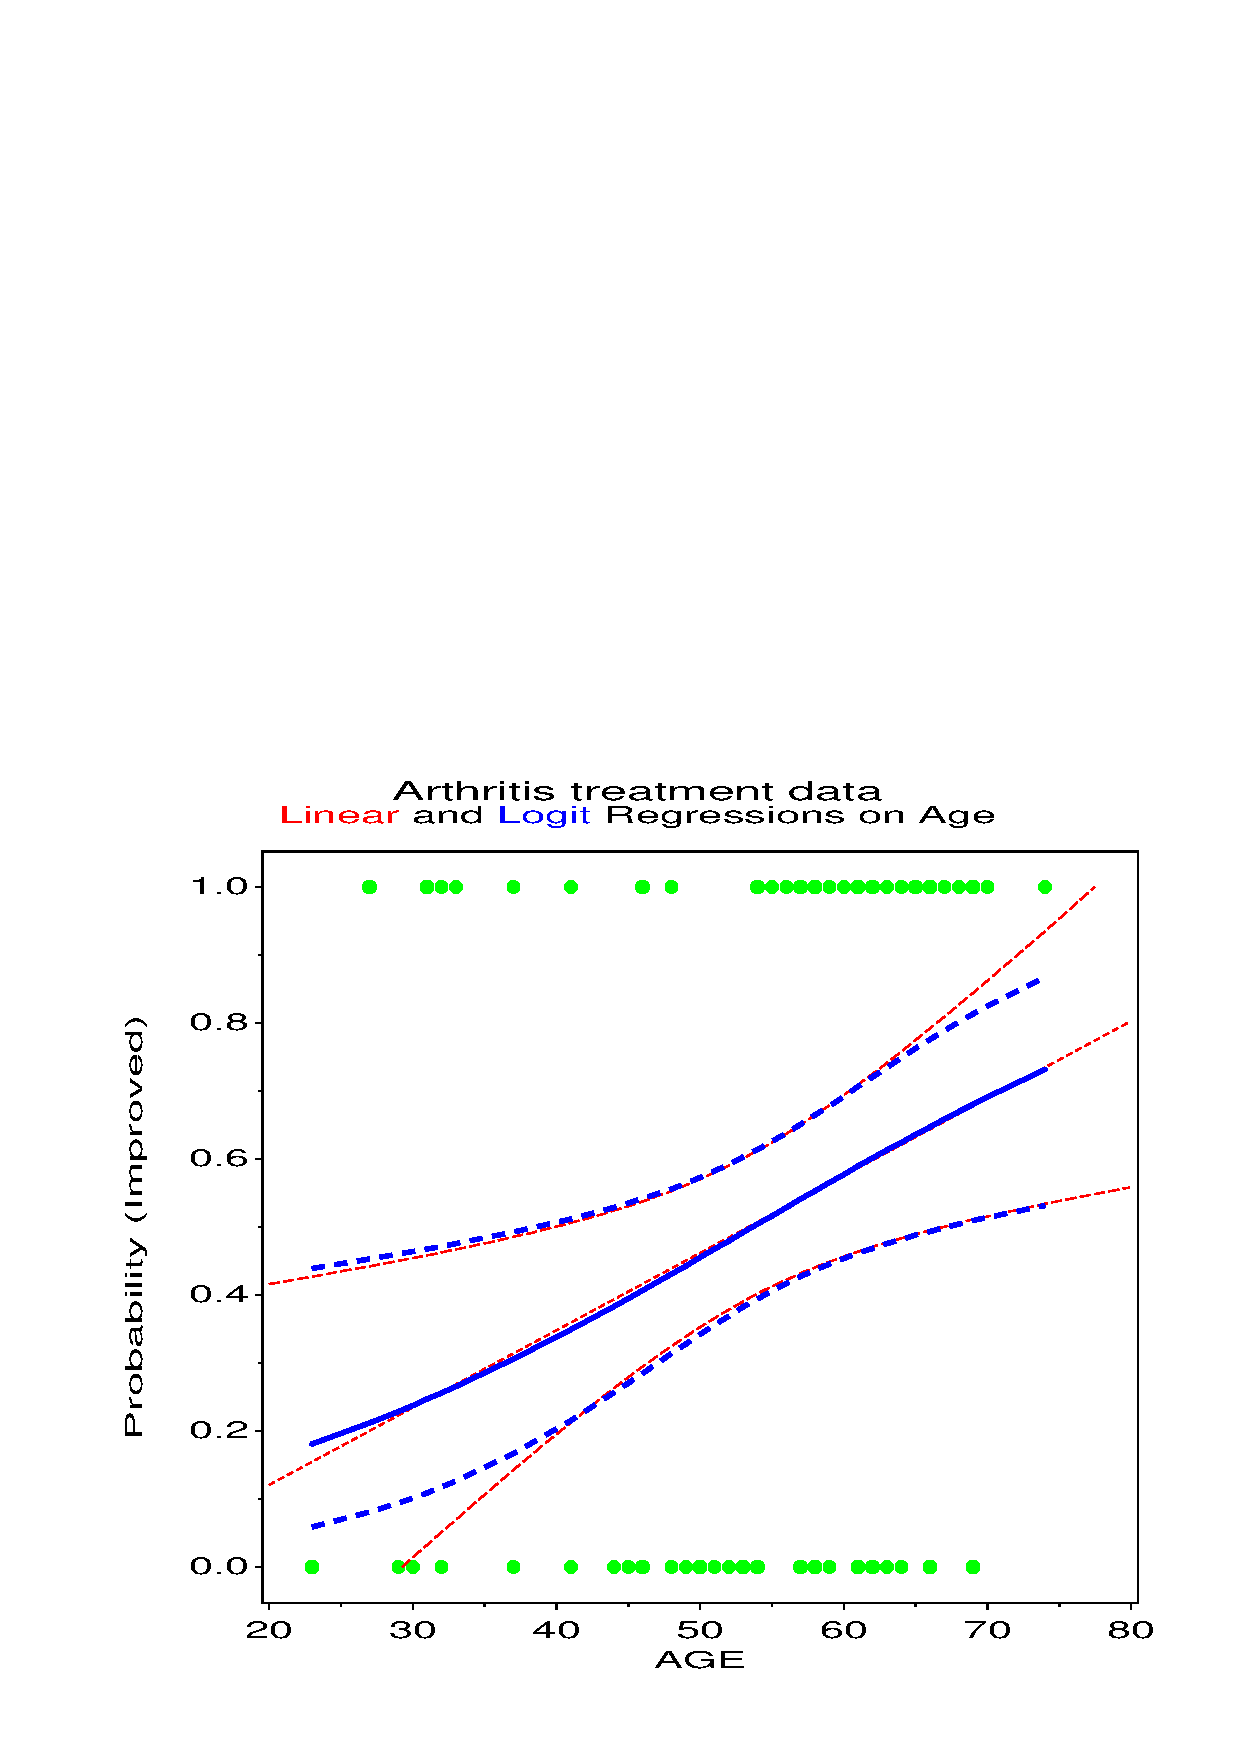
\includegraphics[scale=.7]{ch6/fig/logist1c1}
  \caption[Arthritis treatment data, linear and logit regressions on age]%
  {Arthritis treatment data, linear and logit regressions on age.  The curves show predicted probabilities of
improvement and 95\% confidence bands.
The points show the observations.  Except in the extremes, the linear
and logistic models give very similar predicted values; the confidence bounds
differ more.}%
  \label{fig:logist1c1}
\end{figure}

The relevant portion of the output is shown below.  The parameter estimates
are $\alpha = -2.642$, and $\beta = 0.0492$.  So, the estimated odds of
a better response are multiplied by $e^{\beta} = \exp(0.0492) = 1.05$
for each one year increase in age.  Equivalently, you can think of this
as a 5\% increase per year (using $100 (e^{\beta} -1)$ to convert).
Over 10 years, the odds are multiplied by $\exp(10 \times 0.0492) = 1.64$,
a 64\% increase.
\begin{output}
                  Analysis of Maximum Likelihood Estimates

            Parameter Standard    Wald       Pr >    Standardized    Odds
Variable DF  Estimate   Error  Chi-Square Chi-Square   Estimate     Ratio

INTERCPT 1    -2.6421   1.0732     6.0611     0.0138            .    .
AGE      1     0.0492   0.0194     6.4733     0.0110     0.346714   1.050
\end{output}
\end{Example}
